\documentclass{beamer}
\mode<presentation>

\usepackage[utf8]{inputenc}
\usepackage[T1]{fontenc}
\usepackage[slovene]{babel}
\usepackage{lmodern}
\usepackage{array} 
\usepackage{tikz}

\usetheme{Berlin}
\usecolortheme{default}
\useinnertheme[shadows]{rounded}
\useoutertheme{infolines}
\beamertemplatenavigationsymbolsempty

\usepackage{times}
\newcommand{\ds}{\displaystyle}
\newcommand{\ts}{\textstyle}
\newcommand{\presledek}{\vspace{3mm}}
\newcommand{\ph}{\phantom{1}} 
\newcommand{\tr}{{\rm tr \,}}

\newtheorem{definicija}{Definicija}
\newtheorem{izrek}{Izrek}
\newtheorem{trditev}{Trditev}


\begin{document}

%%%%%%%%%%%%%%%%%%%%%%%%%%%%%%%%%%%%%%%%%%%%%%%%%%%%%%%%%%%%%%%%%%%%%%%%%%%%%%%%%%%%%%%%%%%%%%%%%%%%%%%%%%%%%%%%%%%%%%%%%%%%%%%%%%%%%%%%%%%%
%%%%%%%%%%%%%%%%%%%%%%%%%%%%%%%%%%%%%%%%%%%%%%%%%%%%%%%%%%%%%%%%%%%%%%%%%%%%%%%%%%%%%%%%%%%%%%%%%%%%%%%%%%%%%%%%%%%%%%%%%%%%%%%%%%%%%%%%%%%%
\title{Statistika v kazenskem pravu}
\subtitle{Dolga predstavitev diplomske naloge}
\author[Neža Kržan]{Neža Kržan}
 
\institute[FMF]{Mentor: izr. prof. Jaka Smrekar \\ Fakulteta za matematiko in fiziko \\ \vspace{10mm} Ljubljana, 5.maj 2023}
\date[5. maj 2023] {}

\subject{Talks}

\begin{frame}
   \titlepage
\end{frame}

%%%%%%%%%%%%%%%%%%%%%%%%%%%%%%%%%%%%%%%%%%%%%%%%%%%%%%%%%%%%%%%%%%%%%%%%%%%%%%%%%%%%%%%%%%%%%%%%%%%%%%%%%%%%%%%%%%%%%%%%%%%%%%%%%%%%%%%%%%%%
%%%%%%%%%%%%%%%%%%%%%%%%%%%%%%%%%%%%%%%%%%%%%%%%%%%%%%%%%%%%%%%%%%%%%%%%%%%%%%%%%%%%%%%%%%%%%%%%%%%%%%%%%%%%%%%%%%%%%%%%%%%%%%%%%%%%%%%%%%%%
\begin{frame}
   \frametitle{Kratek pregled}
   \tableofcontents[pausesections]
\end{frame}

%%%%%%%%%%%%%%%%%%%%%%%%%%%%%%%%%%%%%%%%%%%%%%%%%%%%%%%%%%%%%%%%%%%%%%%%%%%%%%%%%%%%%%%%%%%%%%%%%%%%%%%%%%%%%%%%%%%%%%%%%%%%%%%%%%%%%%%%%%%%
%%%%%%%%%%%%%%%%%%%%%%%%%%%%%%%%%%%%%%%%%%%%%%%%%%%%%%%%%%%%%%%%%%%%%%%%%%%%%%%%%%%%%%%%%%%%%%%%%%%%%%%%%%%%%%%%%%%%%%%%%%%%%%%%%%%%%%%%%%%%
\section{Statistika v kazenskem pravu}

\begin{frame}
    \frametitle{Statistika v kazenskem pravu}
    \begin{itemize}
        \item Preverjamo \textbf{teorije} in \textbf{hipoteze}.
        \item Preučujemo razmerja med dvema ali več spremenljivkami.\\ \vspace{2mm}
        \begin{block}{}
            \textbf{Odvisne spremenljivke} - empirični dogodki, ki jih želi raziskovalec pojasniti.\\
            \textbf{Neodvisne spremenljivke} - dejavniki, za katere raziskovalec meni, da bi lahko vplivali na odvisne spremenljivke.
        \end{block}
        \begin{enumerate}
            \item časovno zaporedje;
            \item obstajati mora empirična povezava med odvisno in neodvisno spremenljivko;
            \item razmerje med neodvisno in odvisno spremenljivko nepristransko;
        \end{enumerate}
    \end{itemize}
\end{frame}

%%%%%%%%%%%%%%%%%%%%%%%%%%%%%%%%%%%%%%%%%%%%%%%%%%%%%%%%%%%%%%%%%%%%%%%%%%%%%%%%%%%%%%%%%%%%%%%%%%%%%%%%%%%%%%%%%%%%%%%%%%%%%%%%%%%%%%%%%%%%
\begin{frame}
    \frametitle{Težave}
    \begin{block}{}
        \centering
        Določitev odvisnih in neodvisnih spremenljivk za modeliranje.
    \end{block}
    V proces določanja spremenljivk pogosto posežejo odvetniki, ki se sklicujejo na pravne zakone in načela. To lahko postane sporno, saj lahko takšni 
    posegi ovirajo statistične znanstvenike pri izračunu verjetnostnega vpliva spremenljivk.
\end{frame}

%%%%%%%%%%%%%%%%%%%%%%%%%%%%%%%%%%%%%%%%%%%%%%%%%%%%%%%%%%%%%%%%%%%%%%%%%%%%%%%%%%%%%%%%%%%%%%%%%%%%%%%%%%%%%%%%%%%%%%%%%%%%%%%%%%%%%%%%%%%%
%%%%%%%%%%%%%%%%%%%%%%%%%%%%%%%%%%%%%%%%%%%%%%%%%%%%%%%%%%%%%%%%%%%%%%%%%%%%%%%%%%%%%%%%%%%%%%%%%%%%%%%%%%%%%%%%%%%%%%%%%%%%%%%%%%%%%%%%%%%%
\section{Uporaba statistike pri pravnem postopku}

\begin{frame}
    \frametitle{Uporaba statistike pri pravnem postopku}
    Pred pričanjem na sodišču moramo vedeti
    \begin{enumerate}
        \item na kaj točno se podatki nanašajo,
        \item kako so bili zbrani,
        \item kakšen del manjka ali je neuporaben.
    \end{enumerate}
    $\Rightarrow$ \textbf{Določimo ustrezen postopek analize podatkov.}\\ \vspace{3mm}
    Potrebujemo
    \begin{enumerate}
        \item osnovne informacije odvetnika in drugih strokovnjakov,
        \item določitev ustrezne populacije,
        \item določitev parametrov, ki nas zanimajo,
        \item določitev statističnega postopka.
    \end{enumerate}
    $\Rightarrow$ \textbf{Oblikujemo ustrezne primerjalne skupine.}
\end{frame}

%%%%%%%%%%%%%%%%%%%%%%%%%%%%%%%%%%%%%%%%%%%%%%%%%%%%%%%%%%%%%%%%%%%%%%%%%%%%%%%%%%%%%%%%%%%%%%%%%%%%%%%%%%%%%%%%%%%%%%%%%%%%%%%%%%%%%%%%%%%%%%
%%%%%%%%%%%%%%%%%%%%%%%%%%%%%%%%%%%%%%%%%%%%%%%%%%%%%%%%%%%%%%%%%%%%%%%%%%%%%%%%%%%%%%%%%%%%%%%%%%%%%%%%%%%%%%%%%%%%%%%%%%%%%%%%%%%%%%%%%%%%%%
\section{Raziskovalni proces}
\begin{frame}
    \frametitle{Raziskovalni proces}
    Raziskovalni proces v kazenskem pravosodju je običajno namenjen preučevanju problemov kriminala. Proces se izvaja po naslednjih točkah.\\ \vspace{2mm}
    \begin{enumerate}
        \item \textbf{Identifikacija problema.\\} 
        \item \textbf{Zasnova raziskave.\\} 
        \item \textbf{Analiza podatkov.\\}
    \end{enumerate}
\end{frame}

%%%%%%%%%%%%%%%%%%%%%%%%%%%%%%%%%%%%%%%%%%%%%%%%%%%%%%%%%%%%%%%%%%%%%%%%%%%%%%%%%%%%%%%%%%%%%%%%%%%%%%%%%%%%%%%%%%%%%%%%%%%%%%%%%%%%%%%%%%%%%%
%%%%%%%%%%%%%%%%%%%%%%%%%%%%%%%%%%%%%%%%%%%%%%%%%%%%%%%%%%%%%%%%%%%%%%%%%%%%%%%%%%%%%%%%%%%%%%%%%%%%%%%%%%%%%%%%%%%%%%%%%%%%%%%%%%%%%%%%%%%%%%
\section{Vrednotenje dokazov}
\begin{frame}
    \frametitle{Vrednotenje dokazov}
    \begin{block}{Dokazni standard}
        pravno vprašanje, tj. gre za abstraktno normo, ki je (podobno kot obstoj določenih predpostavk za 
        določeno kaznivo dejanje) opredeljena s pravnim pravilom.
    \end{block}\vspace{3mm}
    \textbf{METODA DOKAZNE VREDNOSTI}\\
    \textbf{MODEL VERJETNOSTI HIPOTEZE}\\ \vspace{3mm}
    V kazenskem pravu lahko zelo hitro pride do posebnih, edinstvenih predpostavk oziroma hipotez, ki pa predstavljajo težave pri vrednotenju oziroma merjenju v statističnih modelih. 
\end{frame}


%%%%%%%%%%%%%%%%%%%%%%%%%%%%%%%%%%%%%%%%%%%%%%%%%%%%%%%%%%%%%%%%%%%%%%%%%%%%%%%%%%%%%%%%%%%%%%%%%%%%%%%%%%%%%%%%%%%%%%%%%%%%%%%%%%%%%%%%%%%%
%%%%%%%%%%%%%%%%%%%%%%%%%%%%%%%%%%%%%%%%%%%%%%%%%%%%%%%%%%%%%%%%%%%%%%%%%%%%%%%%%%%%%%%%%%%%%%%%%%%%%%%%%%%%%%%%%%%%%%%%%%%%%%%%%%%%%%%%%%%%
\section{Koncept verjetnosti}

\begin{frame}
    \frametitle{Koncept verjetnosti}
    Opravlja se primerjava verjetnosti dokazov na podlagi dveh konkurenčnih predlogov:\\
    $H_p \dots$ trditev, ki jo predlaga tožilstvo;\\
    $H_d \dots$ trditev, ki jo predlaga obramba.\\ \vspace{5mm}
    Koncept verjetnosti je
    \begin{itemize}
        \item ključen pri ocenjevanju dokazov;
        \item omogoča objektivno oceno vpliva dokaza na verjetnost določene domneve o interesni osebi ali obdolžencu.
    \end{itemize}
\end{frame}

%%%%%%%%%%%%%%%%%%%%%%%%%%%%%%%%%%%%%%%%%%%%%%%%%%%%%%%%%%%%%%%%%%%%%%%%%%%%%%%%%%%%%%%%%%%%%%%%%%%%%%%%%%%%%%%%%%%%%%%%%%%%%%%%%%%%%%%%%%%%
\begin{frame}
    \frametitle{Presoja dokazov}
    \begin{itemize}
        \item Za presojo se uporablja različne metode in tehnike, ki temeljijo na statistični verjetnosti,
        \item metode omogočajo oceno, kako verjetno je, da so dokazi resnični in zanesljivi. 
    \end{itemize}
    \begin{beamerboxesrounded}[]{KONTEKST DOKAZA}
        \begin{itemize}
            \item Upoštevamo druge dokaze in okoliščine primera.
            \item Izvedemo bolj objektivno presojo dokazov.
            \item Vpliv na določeno domnevo oziroma hipotezo o interesni osebi ali obdolžencu.
            \item Upoštevamo verjetnost napake - verjetnost, da so dokazi napačni ali zavajajoči.
        \end{itemize} 
    \end{beamerboxesrounded}
\end{frame}

%%%%%%%%%%%%%%%%%%%%%%%%%%%%%%%%%%%%%%%%%%%%%%%%%%%%%%%%%%%%%%%%%%%%%%%%%%%%%%%%%%%%%%%%%%%%%%%%%%%%%%%%%%%%%%%%%%%%%%%%%%%%%%%%%%%%%%%%%%%%
\begin{frame}
    \frametitle{Koncept verjetnosti}
    \begin{beamerboxesrounded}[]{Verjetnost proti nedolžnosti ali verjetnost za krivdo}
        \[
            \frac{P(H_p)}{P(H_d)}
        \]    
    \end{beamerboxesrounded} \vspace{3mm}
    \begin{beamerboxesrounded}[]{Verjetnost v prid krivdi ob upoštevanju informacij $E$}
        \[
            \frac{P(H_p \lvert E)}{P(H_d \lvert E)} 
        \]    
    \end{beamerboxesrounded} \vspace{5mm}
    Če imamo na voljo dokaz $E$, nas zanima pogojna verjetnost
    \[
        P(kriv \lvert E), \vspace{2mm}
    \]
    pri čemer nam je lahko v pomoč Bayesovo pravilo.
\end{frame}

%%%%%%%%%%%%%%%%%%%%%%%%%%%%%%%%%%%%%%%%%%%%%%%%%%%%%%%%%%%%%%%%%%%%%%%%%%%%%%%%%%%%%%%%%%%%%%%%%%%%%%%%%%%%%%%%%%%%%%%%%%%%%%%%%%%%%%%%%%%%
%%%%%%%%%%%%%%%%%%%%%%%%%%%%%%%%%%%%%%%%%%%%%%%%%%%%%%%%%%%%%%%%%%%%%%%%%%%%%%%%%%%%%%%%%%%%%%%%%%%%%%%%%%%%%%%%%%%%%%%%%%%%%%%%%%%%%%%%%%%%
\section{Bayesova statistika}

\begin{frame}
    \frametitle{Opredelitev}
    Bayesova statistika je statistična veja, ki nam s pomočjo matematičnih pristopov omogoča uporabo verjetnosti pri reševanju statističnih 
    problemov. V svoje modele vključuje pogojno verjetnost, katero izračunamo z uporabo Bayesovega pravila. \\ \vspace{3mm}
    Hipoteza: Oseba je »kriva«.
    \begin{enumerate}
        \item začnemo z nekim predhodnim prepričanjem o hipotezi;
        \item ga posodabljamo, ko se dokazi ponovno pojavijo.
    \end{enumerate}
\end{frame}


%%%%%%%%%%%%%%%%%%%%%%%%%%%%%%%%%%%%%%%%%%%%%%%%%%%%%%%%%%%%%%%%%%%%%%%%%%%%%%%%%%%%%%%%%%%%%%%%%%%%%%%%%%%%%%%%%%%%%%%%%%%%%%%%%%%%%%%%%%%%
\begin{frame}
    \frametitle{Bayesovo pravilo}
    Bayesovo sklepanje temelji na Bayesovem pravilu, ki izraža verjetnost nekega dogodka z verjetnostjo dveh dogodkov in obrnejnje pogojne
    verjetnosti. \vspace{3mm}
    \begin{definicija}
        Bayesovo pravilo:
        \[
            P(H \lvert E) = \frac{P(E \lvert H) \times P(H)}{P(E)}, \vspace{2mm}
        \] 
    \end{definicija} \vspace{3mm}
    Obstaja še ena formulacija Bayesovega pravila, ki olajša izračune in je pogosto uporabljena pri Bayesovi analizi DNK dokazov
    \[
        \frac{P(H \lvert E)}{P(\neg H \lvert E)} = \frac{P(E \lvert H)}{P(E \lvert \neg H)} \times \frac{P(H)}{P(\neg H)}. \vspace{2mm}
    \]
\end{frame}

%%%%%%%%%%%%%%%%%%%%%%%%%%%%%%%%%%%%%%%%%%%%%%%%%%%%%%%%%%%%%%%%%%%%%%%%%%%%%%%%%%%%%%%%%%%%%%%%%%%%%%%%%%%%%%%%%%%%%%%%%%%%%%%%%%%%%%%%%%%%
\begin{frame}
    \frametitle{Bayesovo posodabljenje}
    Logična trditev, kako se sčasoma posodabljajo apriorne oziroma predhodne verjetnosti dokazov glede na novo zbrane dokaze oziroma prepričanja. \vspace{3mm}
    \begin{trditev}[Bayesovo posodabljanje]
        Če se dogodek E zgodi ob času $t_1 > t_0$, potem je $P_1(H) = P_0(H \lvert E)$.
    \end{trditev}
    \begin{itemize}
        \item Predhodna oz. apriorna verjetnost = $P_0(H)$ (ob času $t_0$ dogodku H dodelimo verjetnost);
        \item Ko se zgodi dogodek E ob času $t_1$, ki vpliva na naša prepričanja o dogodku H, Bayesovo posodabljanje pravi, da je potrebno apriorno 
        verjetnost dogodka H v času $t_1$ enačiti z pogojno verjetnostjo dogodka H glede na dogodek E v času $t_0$. 
    \end{itemize}
\end{frame}

%%%%%%%%%%%%%%%%%%%%%%%%%%%%%%%%%%%%%%%%%%%%%%%%%%%%%%%%%%%%%%%%%%%%%%%%%%%%%%%%%%%%%%%%%%%%%%%%%%%%%%%%%%%%%%%%%%%%%%%%%%%%%%%%%%%%%%%%%%%%
\begin{frame}
    \frametitle{Bayesova teorija v kazenskem pravu}
    Bayesovo sklepanje razlaga verjetnost kot merilo verjetnosti ali zaupanja, ki ga lahko ima posameznik glede nastanka določenega dogodka.
    \begin{itemize}
      \item O dogodku lahko že imamo predhodno prepričanje oziroma apriorno prepričanje.
      \item Ta se lahko spremeni, ko se pojavijo novi dokazi.
    \end{itemize} \vspace{3mm}
    Bayesova statistika nam daje matematične modele za vključevanje naših apriornih prepričanj in dokazov za ustvarjanje novih prepričanj.
\end{frame}

\begin{frame}
    \frametitle{Bayesova teorija v kazenskem pravu}
    Ocena, kako informacije vplivajo na tožilčevo domnevo o obdolžencu oziroma storilcu kaznivega dejanja. \\ \vspace{3mm}
    Postopek posodabljanja verjetnosti tožilčeve hipoteze na podlagi predhodnih oziroma apriornih verjetnosti. \\ \vspace{3mm}
    \begin{block}{}
        \centering
        verjetnost hipoteze pred upoštevanjem določenega dokaza (dokazov) \\ \vspace{2mm}
        $\Rightarrow$ \\ \vspace{3mm}
        verjetnost hipoteze po upoštevanju določenega dokaza (dokazov)
    \end{block}
\end{frame}

%%%%%%%%%%%%%%%%%%%%%%%%%%%%%%%%%%%%%%%%%%%%%%%%%%%%%%%%%%%%%%%%%%%%%%%%%%%%%%%%%%%%%%%%%%%%%%%%%%%%%%%%%%%%%%%%%%%%%%%%%%%%%%%%%%%%%%%%%%%%
\begin{frame}
    \frametitle{Predhodna verjetnost in določitev posteriorne verjetnosti}
    Recimo, da je statistični znanstvenik naprošen, da opravi analizo profila DNK krvi, najdene na kraju kaznivega dejanja, in rezultat primerja s profilom DNK 
    obdolženca.\\ \vspace{3mm}
    Odločitev porotnikov bo delno odvisna od njihove ocene dveh interesnih
    hipotez\\
    $H_1 \dots$ vir krvi je obtoženec,\\
    $H_2 \dots$ vir krvi je druga oseba.\\ \vspace{3mm}
    Porotniki bodo morda želeli, da jim dokončno povemo, katera hipoteza je resnična, ali da jim navedemo verjetnosti vira. Za oceno verjetnosti 
    vira mora statistični znanstvenik upoštevati tudi druge dokaze v kazenskem primeru.
\end{frame}

\begin{frame}
    \frametitle{Predhodna verjetnost in določitev posteriorne verjetnosti}
    Obtoženec in kri s kraja zločina imata skupen niz t.i. genetskih označevalcev - najdemo pri eni osebi na 1 milijon prebivalcev.\\ \vspace{3mm}
    \centering
    $\rightarrow$ \textbf{pogojna verjetnost ugotovitve rezultatov pri dveh hipotezah o medsebojni povezanosti}
    \begin{itemize}
        \item skupni genetski označevalci skoraj zagotovo najdeni v primeru $H_1$ (vir je bil obtoženec);
        \item 1 možnost na milijon, da bodo najdeni v primeru $H_2$ (vir je bil nekdo drug);
    \end{itemize}
    \centering 
    $\rightarrow$ \textbf{predložimo razmerje verjetnosti}
\end{frame}

%%%%%%%%%%%%%%%%%%%%%%%%%%%%%%%%%%%%%%%%%%%%%%%%%%%%%%%%%%%%%%%%%%%%%%%%%%%%%%%%%%%%%%%%%%%%%%%%%%%%%%%%%%%%%%%%%%%%%%%%%%%%%%%%%%%%%%%%%%%%
\begin{frame}
    \frametitle{Težave z določitvijo predhodne verjetnosti}
    Različne metode za določitev in izračun predhodnih verjetnosti lahko dajejo različne rezultate. \\ \vspace{3mm}
    \begin{block}{Ali naj analitiki poskušajo določiti predhodne verjetnosti in če ja, kako naj jih določijo?}
        \begin{itemize}
            \item \textbf{Nevtralno stanje} - analitiki predpostavi enake predhodne verjetnosti za vse hipoteze v primeru;
            \item Analitik naj uporabi svoje strokovno znanje za izračun apriorne verjetnosti na podlagi razpoložljivih podatkov in brez nepotrebnega vplivanja odvetnikov ali drugih udeležencev postopka;
        \end{itemize}
    \end{block}
\end{frame}

%%%%%%%%%%%%%%%%%%%%%%%%%%%%%%%%%%%%%%%%%%%%%%%%%%%%%%%%%%%%%%%%%%%%%%%%%%%%%%%%%%%%%%%%%%%%%%%%%%%%%%%%%%%%%%%%%%%%%%%%%%%%%%%%%%%%%%%%%%%%
%%%%%%%%%%%%%%%%%%%%%%%%%%%%%%%%%%%%%%%%%%%%%%%%%%%%%%%%%%%%%%%%%%%%%%%%%%%%%%%%%%%%%%%%%%%%%%%%%%%%%%%%%%%%%%%%%%%%%%%%%%%%%%%%%%%%%%%%%%%%
\section{Bayesova analiza}

\begin{frame}
    \frametitle{Poenostavljena Bayesova analiza}
    Naj bo:\\
    $S$ \dots trditev, da je obtoženec vir sledi DNK s kraja zločina; \\
    $M$ \dots trditev, da se obtoženčev DNK ujema z DNK-jem s kraja zločina; \\
    $f$ \dots funkcija pogostosti ujemanja DNK z DNK-jem s kraja zločina. \\
    Želimo vedeti, kakšna je verjetnost S glede na M, tj. $P(S \lvert M)$. \\ \vspace{3mm}
    Bayesovo pravilo lahko uporabimo na naslednji način:
    \[
        \frac{P(S \lvert M)}{P(\neg S \lvert M)} = \frac{P(M \lvert S)}{P(M \lvert \neg S)} \times \frac{P(S)}{P(\neg S)}.
    \] 
\end{frame} 

\begin{frame}
    \frametitle{Poenostavljena Bayesova analiza}
    \[
        \frac{P(S \lvert M)}{P(\neg S \lvert M)} = \frac{P(M \lvert S)}{P(M \lvert \neg S)} \times \frac{P(S)}{P(\neg S)}. \vspace{3mm}
    \] 
    \begin{block}{}
        \centering
        $P(M \lvert S) = 1$ - \textbf{lažno negativni rezultat};\\ \vspace{2mm}
        $P(M \lvert \neg S) = f$ - \textbf{lažno pozitivni rezultat}; 
    \end{block}
\end{frame}

%%%%%%%%%%%%%%%%%%%%%%%%%%%%%%%%%%%%%%%%%%%%%%%%%%%%%%%%%%%%%%%%%%%%%%%%%%%%%%%%%%%%%%%%%%%%%%%%%%%%%%%%%%%%%%%%%%%%%%%%%%%%%%%%%%%%%%%%%%%%
\begin{frame}
    \frametitle{Izpopolnjena Bayesova analiza l}
    Za upoštevanje možnosti laboratorijskih napak, bomo namesto $M$ uvedli spremenljivko $M_p$.\\ \vspace{3mm}
    $M_p$ \dots poročano ujemanje laboratorijske analize; \\ 
    $M_t$ \dots trditev, da obstaja dejansko ujemanje v DNK-ju;\\
    $\neg M_t$ \dots trditev, da obstaja neujemanje v DNK-ju.  \\ 
    $f$ \dots pogostost ujemnja DNK-ja z DNK-jem s kraja zložina;\\
    $P(M_t \lvert \neg S) = f$; \\
    $P(\neg M_t \lvert \neg S) = 1-f$;\\
    $P(M_p \lvert \neg M_t)$ \dots opisuje verjetnost lažno pozitivnih rezultatov laboratorija(oznaka $FP$);\\
    $P(M_p \lvert M_t)$ \dots opisuje verjetnost resničnih pozitivnih rezultatov laboratorija(oznaka $FN$).\\\vspace{3mm}
    Sledi:
    \[
        P(M \lvert \neg S) = [(1 - FN) \times f] + [FP \times (1 - f)]. \vspace{2mm}
    \]
\end{frame}
 
\begin{frame}
    \frametitle{Izpopolnjena Bayesova analiza}
    \begin{itemize}
        \item Relativno majhne stopnje napak lahko bistveno zmanjšajo dokazno vrednost DNK dokazov, saj močno zmanjšajo razmerje verjetnosti.
        \item Vpliv stopnje laboratorijskih napak kaže, da ne glede na to, kako nizka se izkaže pogostost profila, bo ta relativno nepomembna, če pogostosti ne spremlja ocena stopnje laboratorijskih napak.
    \end{itemize} \vspace{3mm}
    Spremenljivost pogostosti profila lahko v Bayesovem okviru upoštevamo na dva načina: 
    \begin{enumerate}
        \item s spremembo predhodne verjetnosti;
        \item s spremembo pogostosti profila.
    \end{enumerate}
\end{frame}

%%%%%%%%%%%%%%%%%%%%%%%%%%%%%%%%%%%%%%%%%%%%%%%%%%%%%%%%%%%%%%%%%%%%%%%%%%%%%%%%%%%%%%%%%%%%%%%%%%%%%%%%%%%%%%%%%%%%%%%%%%%%%%%%%%%%%%%%%%%%
%%%%%%%%%%%%%%%%%%%%%%%%%%%%%%%%%%%%%%%%%%%%%%%%%%%%%%%%%%%%%%%%%%%%%%%%%%%%%%%%%%%%%%%%%%%%%%%%%%%%%%%%%%%%%%%%%%%%%%%%%%%%%%%%%%%%%%%%%%%%
\section{Drugi pristopi}

\begin{frame}
    \frametitle{Frekvence}
    \begin{itemize}
        \item frekvence se običajno nanašajo na pojavljanje dokazov za posamezen primer;
        \item sklepanje o krivdi je lahko podprto s verjetnostnim sklepanjem z uporabo absolutnih ali relativnih frekvenc;
    \end{itemize}
    \begin{block}{Relativne frekvence}
        \begin{itemize}
            \item navajajo (predpostavljajo) obstoj referenčnega vzorca, na podlagi katerega se lahko oceni pogostost zadevnega dogodka;
            \item lahko podpre vmesno sklepanje o moči dokazov;
            \item rutinsko vključene v znanstvene dokaze.
        \end{itemize}  
    \end{block}
\end{frame}

\begin{frame}
    \frametitle{Frekvence - obtoženec vir DNK-ja s kraja zločina}
    Recimo, da je pogostost profila DNK $f$ 1 proti 10 milijonov, predpostavimo tudi, da ima obtoženec enak DNK in da je začetna populacija osumljencev 100 milijonov ljudi.
    \begin{block}{}
        \textbf{Kakšna je verjetnost, da je obtoženec vir DNK-ja s kraja zločina?}
    \end{block} \vspace{3mm}
    $f$ \dots pogostost profila DNK;\\
    $m$ \dots velikost populacije osumljencev; \\
    $n$ \dots število ljudi, ki imajo ustrezen DNK profil. \\
    \begin{block}{}
        Potrebno je izračunati, koliko ljudi z zadevnim profilom DNK je v populaciji osumljencem, tako da se $f$ pomnoži z $m$.
    \end{block} 
\end{frame}

\begin{frame}
    \frametitle{Frekvence - obtoženec vir DNK-ja s kraja zločina}
    \begin{enumerate}
        \item $n \ge 1$ $\Rightarrow$ $P(\text{obtoženi je vir})=\frac{1}{n}$
        \item $n < 1$ $\Rightarrow$ frekvence še posebaj majhne
    \end{enumerate} \vspace{3mm}
    \begin{block}{Verjetnost, da ima točno en posameznik ustrezen DNK profil, ob pogoju da ga ima vsaj en posameznik}
        \[
            P(n = 1 \lvert n \ge 1) = \frac{P(n=1 \cap n \ge 1)}{P(n \ge 1)} = \frac{m \times f \times (1 - f)^{m-1}}{1 - (1 - f)^m}
        \]
    \end{block}
\end{frame}

%%%%%%%%%%%%%%%%%%%%%%%%%%%%%%%%%%%%%%%%%%%%%%%%%%%%%%%%%%%%%%%%%%%%%%%%%%%%%%%%%%%%%%%%%%%%%%%%%%%%%%%%%%%%%%%%%%%%%%%%%%%%%%%%%%%%%%%%%%%%
\begin{frame}
    \frametitle{Primerjava z Bayesovo metodo}
    \begin{itemize}
        \item \textbf{metoda edinstvenosti} - ni mogoče enostavno upoštevati številnih zapletov (npr. vpliv stopnje laboratorijskih napak);
        \item Bayesovo pravilo pa omogoča upoštevanje različnih dejavnikov\\ $\rightarrow$ natančni izračuni in bolj zanesljivi rezultati;
        \item \textbf{frekvenčni modeli} - za dokaze, ki jih je mogoče uporabiti za prikaz, kako verjetno je, da bi se naključno izbrana oseba ujemala z vzorcem;
    \end{itemize} \vspace{3mm}
    \begin{block}{}
        \centering
        Izbira metode je odvisna od specifičnih zahtev problema.
    \end{block}
\end{frame}

%%%%%%%%%%%%%%%%%%%%%%%%%%%%%%%%%%%%%%%%%%%%%%%%%%%%%%%%%%%%%%%%%%%%%%%%%%%%%%%%%%%%%%%%%%%%%%%%%%%%%%%%%%%%%%%%%%%%%%%%%%%%%%%%%%%%%%%%%%%%
\begin{frame}
    \frametitle{Metoda verjetnosti naključnega ujemanja}
    \begin{block}{}
        Izraža možnost, da bi imel naključni posameznik, ki ni povezan z obdolžencem, ustrezni DNK profil. Ta verjetnost je enaka pogostosti profila DNK. 
    \end{block}\vspace{2mm}
    Pogosto se to verjetnost interpretira kot:
    \begin{enumerate}
        \item če je verjetnost naključnega ujemanja na primer 1 proti 100 milijonom, potem je verjetnost, da ima profil DNK drug posameznik in ne
        obdolženec 1 proti 100 milijonom;
        \item ker je to zelo majhna verjetnost, mora biti tudi verjetnost, da je sled DNK pustil nekdo drug na kraju zločina in ne obdolženec, zelo majhna;
        \item zato mora biti verjetnost, da je vir sledi DNK s kraja zločina obtoženec zelo velika, ampak znaša 1 proti 100 milijonov.
    \end{enumerate}
\end{frame}

\begin{frame}
    \frametitle{Metoda verjetnosti naključnega ujemanja}
    \begin{block}{}
        \centering
        $\Rightarrow$ \textbf{TOŽILČEVA ZMOTA}
    \end{block} \vspace{2mm}
    \[
        1 - f = P(S \lvert M). \vspace{2mm}
    \]
     Zmota se pojavi v koraku (2), ko je zamenjano $P(M \lvert \neg S)$ s $P(\neg S \lvert M)$ in predpostavljeno, da sta obe verjetnosti enaki $f$. \\\vspace{2mm}
     Namesto verjetnosti naključnega ujemanja forenzični strokovnjaki pogosto pričajo o razmerju verjetnosti dokazov DNK:
     \[
        P(M \lvert S) = P(M \lvert \neg S). \vspace{2mm}
     \] 
\end{frame}

%%%%%%%%%%%%%%%%%%%%%%%%%%%%%%%%%%%%%%%%%%%%%%%%%%%%%%%%%%%%%%%%%%%%%%%%%%%%%%%%%%%%%%%%%%%%%%%%%%%%%%%%%%%%%%%%%%%%%%%%%%%%%%%%%%%%%%%%%%%%
%%%%%%%%%%%%%%%%%%%%%%%%%%%%%%%%%%%%%%%%%%%%%%%%%%%%%%%%%%%%%%%%%%%%%%%%%%%%%%%%%%%%%%%%%%%%%%%%%%%%%%%%%%%%%%%%%%%%%%%%%%%%%%%%%%%%%%%%%%%%
\section{Razmerje verjetnosti}

\begin{frame}
    \frametitle{Opredelitev}
    \begin{definicija}
        Razmerje
        \[
            \frac{P(E \lvert H)}{P(E \lvert \bar{H})} \vspace{2mm}
        \] 
         se imenuje \textbf{razmerje verjetnosti}.
     \end{definicija} \vspace{2mm}
    $\frac{P(H)}{P(\bar{H})}$ \dots predhodna verjetnost v korist H;\\ \vspace{2mm}
    $\frac{P(H \lvert E)}{P(\bar{H} \lvert E)}$ \dots posteriorna verjetnost v korist $H$;
     \begin{block}{}
        Torej iz Bayesovega izreka neposredno izhaja, da če je razmerje verjetnosti 
        \begin{enumerate}
            \item večje od 1, potem dokaz povečuje verjetnost krivde,
            \item če pa je manjše od 1, zmanjšuje verjetnost krivde.
        \end{enumerate}
     \end{block}
\end{frame}

%%%%%%%%%%%%%%%%%%%%%%%%%%%%%%%%%%%%%%%%%%%%%%%%%%%%%%%%%%%%%%%%%%%%%%%%%%%%%%%%%%%%%%%%%%%%%%%%%%%%%%%%%%%%%%%%%%%%%%%%%%%%%%%%%%%%%%%%%%%%
\begin{frame}
    \frametitle{Razmerje verjetnosti v kazenskem pravu}
    $H_p \dots$ interesna oseba(PoI) oz. obtoženec je resnično kriv - nadomestimo $H$;\\
    $H_d \dots$ interesna oseba(PoI) je resnično nedolžen - nadomestimo $\bar{H}$;\\
    $Ev \dots$ obravnavani dokaz - nadomestimo dogodek $E$;\\
    \begin{block}{Bayesovov izreka omogoča, da se predhodne verjetnosti v korist krivde posodobijo v posteriorne verjetnosti}
        \[
            \frac{P(H_p \lvert Ev)}{P(H_d \lvert Ev)} = \frac{P(Ev \lvert H_p)}{P(Ev \lvert H_d)} \times \frac{P(H_p)}{P(H_d)}. \vspace{2mm}
        \]
    \end{block}\vspace{2mm}
    \begin{block}{Ob upoštevanju informacij $I$}
        \[
            \frac{P(H_p \lvert Ev, I)}{P(H_d \lvert Ev, I)} = \frac{P(Ev \lvert H_p, I)}{P(Ev \lvert H_d, I)} \times \frac{P(H_p \lvert I)}{P(H_d \lvert I)}. \vspace{2mm}
        \]
    \end{block}
\end{frame}

\begin{frame}
    \frametitle{Razmerje verjetnosti v kazenskem pravu}
    \begin{definicija}
        Naj bosta  $H_p$ in $H_d$ dve konkurenčni hipotezi ter $I$ informacije o ozadju. Vrednost $V$ dokaza $Ev$ je podana z
        \[
            V = \frac{P(Ev \lvert H_p, I)}{P(Ev \lvert H_d, I)},
        \]
        razmerje verjetnosti, ki pretvori predhodne verjetnosti
        \[
            \frac{P(H_p \lvert I)}{P(H_d \lvert I)} 
        \]
        v posteriorne verjetnosti
        \[
            \frac{P(H_p \lvert Ev, I)}{P(H_d \lvert Ev, I)}.
        \]
     \end{definicija}     
\end{frame}

%%%%%%%%%%%%%%%%%%%%%%%%%%%%%%%%%%%%%%%%%%%%%%%%%%%%%%%%%%%%%%%%%%%%%%%%%%%%%%%%%%%%%%%%%%%%%%%%%%%%%%%%%%%%%%%%%%%%%%%%%%%%%%%%%%%%%%%%%%%%
\begin{frame}
    \frametitle{Utemeljitev uporabe razmerja verjetnosti}
    \begin{enumerate}
        \item katera hipoteza je bolje podprta z dokazi;
        \item v primerih, ko je treba združiti več hipotez in/ali več dokazov;
        \item za količinsko ovrednotenje skupnega učinka več dokazov, ki vključujejo različne povezane hipoteze;
    \end{enumerate} \vspace{3mm}
    \begin{block}{Negotovosti}
        \begin{itemize}
            \item kakovost podatkov, pridobljenih z analizami;
            \item izbira kontrolnega vzorca;
            \item osebno poznavanje okoliščin iz določenega primera;
            \item pridobivanje predhodnih verjetnosti, pogojenih z razpoložljivim znanjem;
            \item numerični postopki za razreševanje računskih težav;
        \end{itemize}
    \end{block} \vspace{2mm}
    \centering
    $\Rightarrow$ \textbf{poročilo vključuje merilo njegove natančnosti}
\end{frame}

%%%%%%%%%%%%%%%%%%%%%%%%%%%%%%%%%%%%%%%%%%%%%%%%%%%%%%%%%%%%%%%%%%%%%%%%%%%%%%%%%%%%%%%%%%%%%%%%%%%%%%%%%%%%%%%%%%%%%%%%%%%%%%%%%%%%%%%%%%%%
\begin{frame}
    \frametitle{Bayesov faktor in razmerje verjetnosti}
    \begin{block}{Bayesov faktor je glavni element Bayesove metodologije za primerjavo konkurenčnih predlogov.}
        \begin{itemize}
            \item sprememba, ki jo povzročijo novi dokazi (podatki) v verjetnosti pri prehodu od predhodne k posteriorni porazdelitvi v korist enega predloga k drugemu;
            \item razmerje verjetnosti poseben primer Bayesovega faktorja;
            \item razmerje dveh mejnih verjetnosti pri konkurenčnih hipotezah;
        \end{itemize}
    \end{block}
\end{frame}

%%%%%%%%%%%%%%%%%%%%%%%%%%%%%%%%%%%%%%%%%%%%%%%%%%%%%%%%%%%%%%%%%%%%%%%%%%%%%%%%%%%%%%%%%%%%%%%%%%%%%%%%%%%%%%%%%%%%%%%%%%%%%%%%%%%%%%%%%%%%
%%%%%%%%%%%%%%%%%%%%%%%%%%%%%%%%%%%%%%%%%%%%%%%%%%%%%%%%%%%%%%%%%%%%%%%%%%%%%%%%%%%%%%%%%%%%%%%%%%%%%%%%%%%%%%%%%%%%%%%%%%%%%%%%%%%%%%%%%%%%
\section{Zmote v kazenskem pravu}
\begin{frame}
    \frametitle{Zmote v kazenskem pravu}
  Številne zmote so zlasti posledica napačnega razumevanja pogojne verjetnosti.
  \begin{itemize}
    \item \textbf{Tožilčeva zmota (angl. Prosecutor’s fallacy)},
    \item \textbf{Zmota obrambnega odvetnika (angl. Defense attorney's fallacy)} in 
    \item \textbf{Zasliševalčeva zmota (angl. Interrogator’s fallacy)}. \vspace{3mm}
  \end{itemize}
\end{frame}

\begin{frame}
    \frametitle{Zmote v kazenskem pravu}
    Če upoštevamo vzročno verigo dokazov, predstavljeno na sliki, lahko razvrstitev zmot posplošimo na večino vrst dokazov. 
    \begin{figure}[!ht]\label{fig:slika_3}
        \centering
        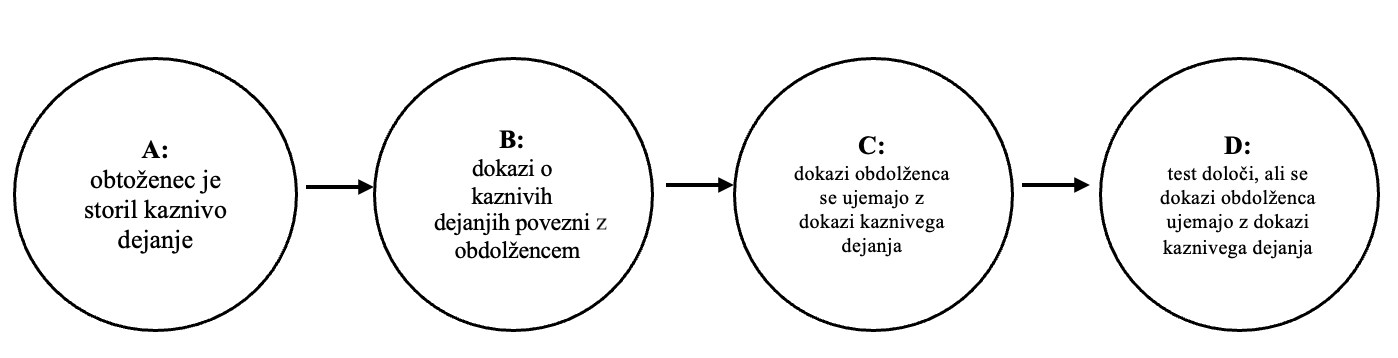
\includegraphics[scale=0.50]{slika_3.png}
        \caption{Vzorčna veriga dokazov}
    \end{figure}
\end{frame}

\begin{frame}
    \frametitle{Zmote v kazenskem pravu}
    \begin{block}{Tožilčeva zmota}
        enačimo $P(C \lvert \neg B)$ s $P(\neg A \lvert C)$
    \end{block}
    \begin{figure}[!ht]\label{fig:slika_3}
        \centering
        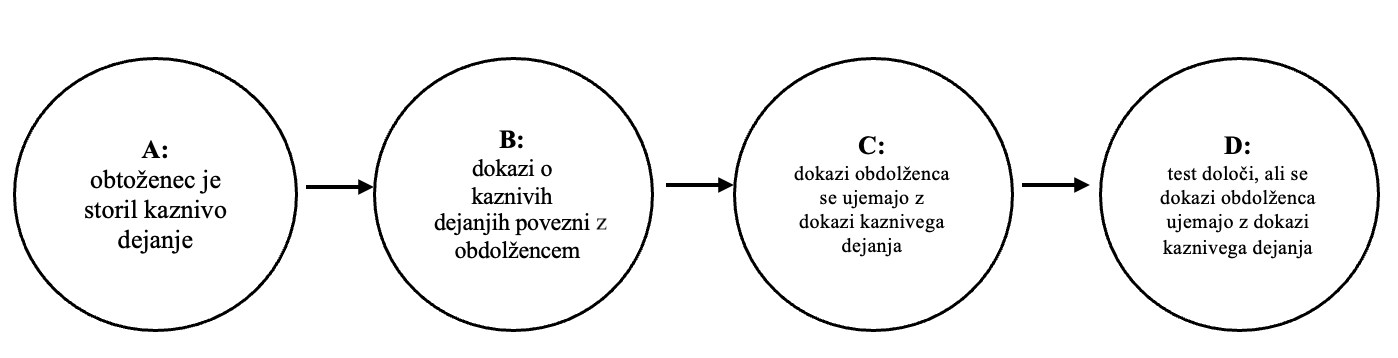
\includegraphics[scale=0.50]{slika_3.png}
        \caption{Vzorčna veriga dokazov}
    \end{figure}
\end{frame}

\begin{frame}
    \frametitle{Zmote v kazenskem pravu}
    \begin{block}{Napaka verjetnosti}
        $P(C \lvert \neg B)$ enačimo z verjetnostjo (imenujmo jo $q$), da ima vsaj en nedolžen član populacije ustreza dokazom
    \end{block}
    \begin{figure}[!ht]\label{fig:slika_3}
        \centering
        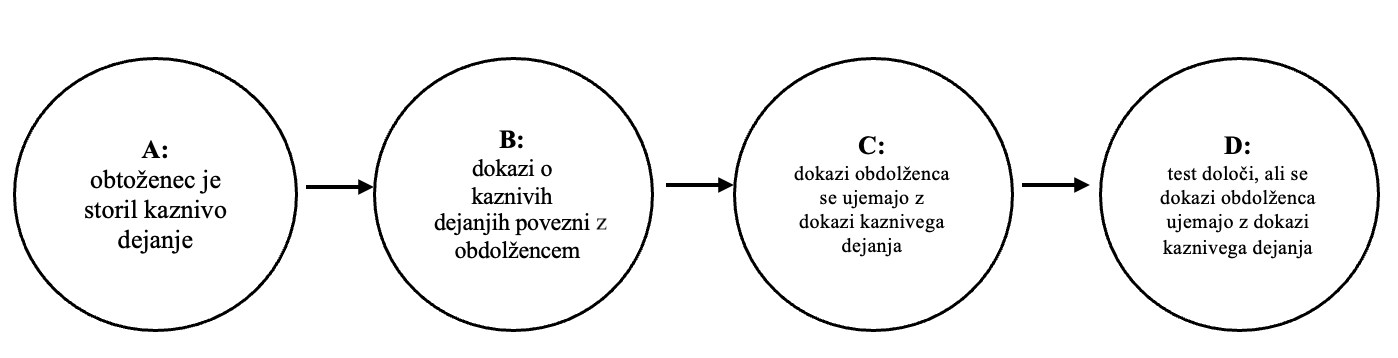
\includegraphics[scale=0.50]{slika_3.png}
        \caption{Vzorčna veriga dokazov}
    \end{figure}
\end{frame}

\begin{frame}
    \frametitle{Zmote v kazenskem pravu}
    \begin{block}{Zanemarjanje predhodnih verjetnosti}
        neupoštevanje predhodnih vrednosti, kot sta $P(A)$ in $P(B)$
    \end{block}
    \begin{figure}[!ht]\label{fig:slika_3}
        \centering
        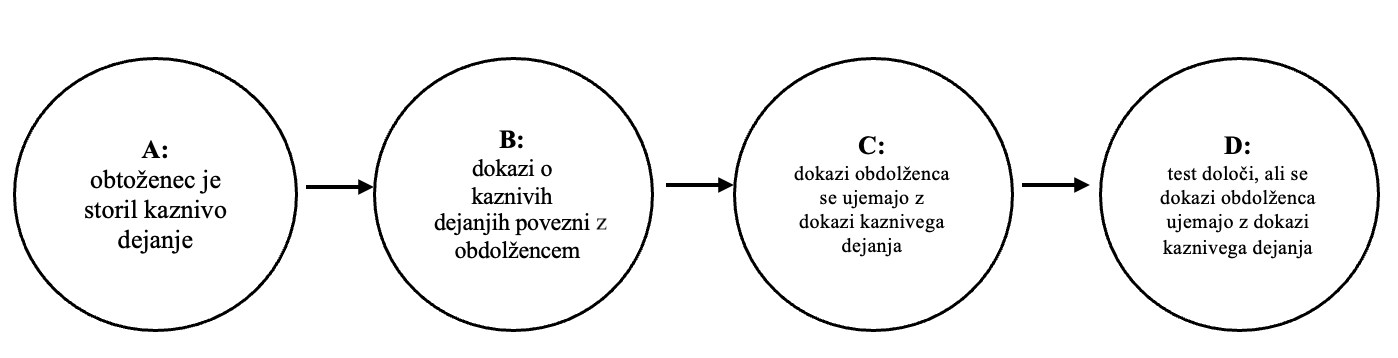
\includegraphics[scale=0.50]{slika_3.png}
        \caption{Vzorčna veriga dokazov}
    \end{figure}
\end{frame}

\begin{frame}
    \frametitle{Zmote v kazenskem pravu}
    \begin{block}{Napaka pri številčnem preračunavanju}
        gre za zamenjavo vrednosti $P(C \lvert \neg B)$ s pričakovanim številom drugih oseb, i bi jih bilo treba testirati, preden bi našli ujemanje
    \end{block}
    \begin{figure}[!ht]\label{fig:slika_3}
        \centering
        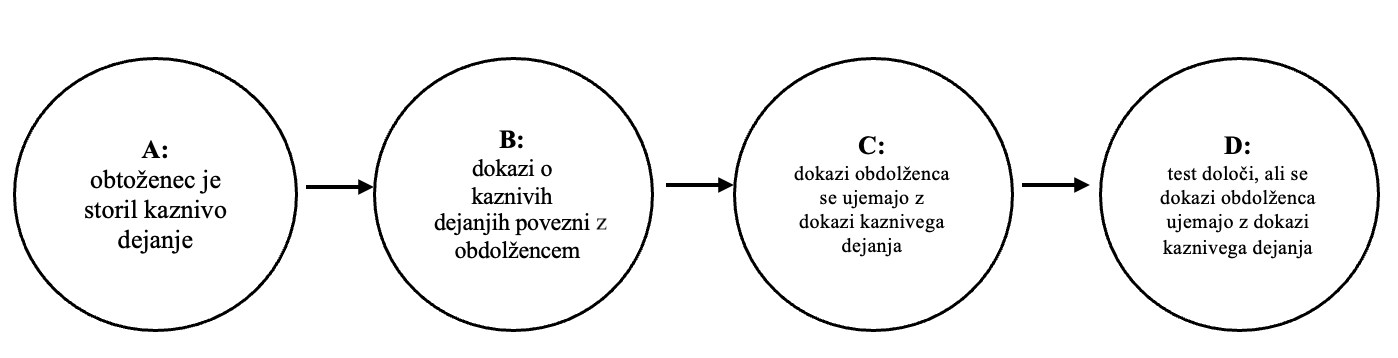
\includegraphics[scale=0.50]{slika_3.png}
        \caption{Vzorčna veriga dokazov}
    \end{figure}
\end{frame}

\begin{frame}
    \frametitle{Zmote v kazenskem pravu}
    \begin{block}{Pričakovane vrednosti, ki pomenijo edinstvenost}
        če je velikost populacije približno enaka $1/P(\neg B \lvert C)$, potem mora biti
        obdolženec edini primerek. Binomski izrek pokaže, da obstaja več kot 25\% verjetnost, da bosta v populaciji, katere velikost je $1/P(\neg B \lvert C)$,
        vsaj dva ujemanja    
    \end{block}
    \begin{figure}[!ht]\label{fig:slika_3}
        \centering
        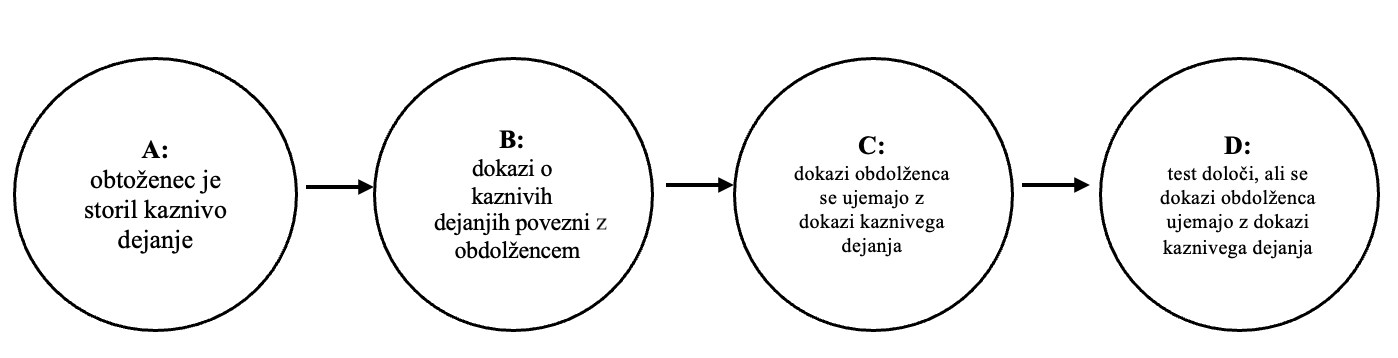
\includegraphics[scale=0.50]{slika_3.png}
        \caption{Vzorčna veriga dokazov}
    \end{figure}
\end{frame}

\begin{frame}
    \frametitle{Zmote v kazenskem pravu}
    \begin{block}{Zmota obrambnega odvetnika}
        dokaz $C$ štejemo za nepomembnega, ker visoka predhodna verjetnost $P(\neg A)$ še vedno povzroči visoko verjetnost $P(\neg B \lvert C)$    
    \end{block}
    \begin{figure}[!ht]\label{fig:slika_3}
        \centering
        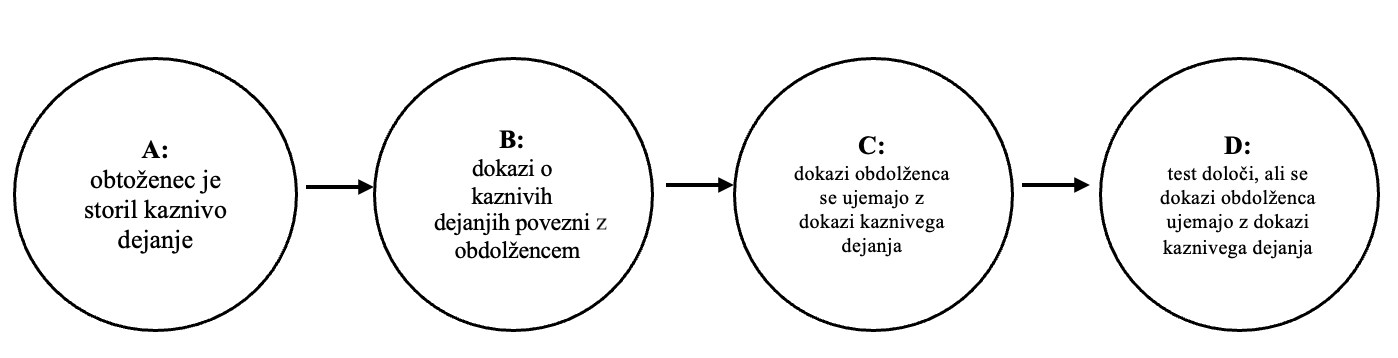
\includegraphics[scale=0.50]{slika_3.png}
        \caption{Vzorčna veriga dokazov}
    \end{figure}
\end{frame}

\begin{frame}
    \frametitle{Zmote v kazenskem pravu}
    \begin{block}{Napaka baze podatkov obrambnega odvetnika}
        verjetnost $P(\neg B \lvert C)$ temelji na drugačni populaciji, kot jo določa $P(B)$ ali $P(A)$    
    \end{block}
    \begin{figure}[!ht]\label{fig:slika_3}
        \centering
        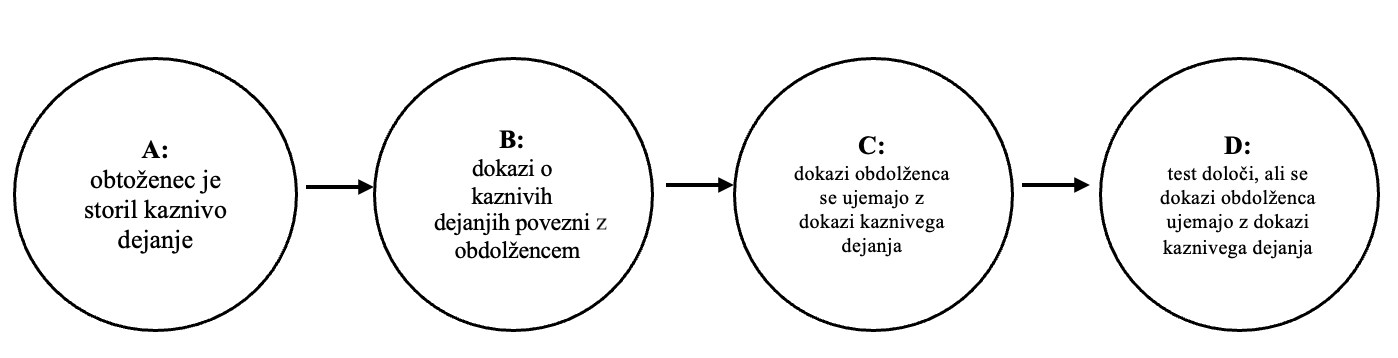
\includegraphics[scale=0.50]{slika_3.png}
        \caption{Vzorčna veriga dokazov}
    \end{figure}
\end{frame}

\begin{frame}
    \frametitle{Zmote v kazenskem pravu}
    \begin{block}{Zasliševalčeva zmota}
        v tem primeru je dokaz neposredno priznanje krivde. Če to ni potrjeno, to pomeni, da uporabljamo $P(D \lvert A)$ za
        informiranje $P(A \lvert D)$. Napaka je, da ne upoštevamo $P(D \lvert \neg A)$. Če je $P(D \lvert A) \leq P(D \lvert \neg A)$, potem dokaz
        nima vrednosti.    
    \end{block}
    \begin{figure}[!ht]\label{fig:slika_3}
        \centering
        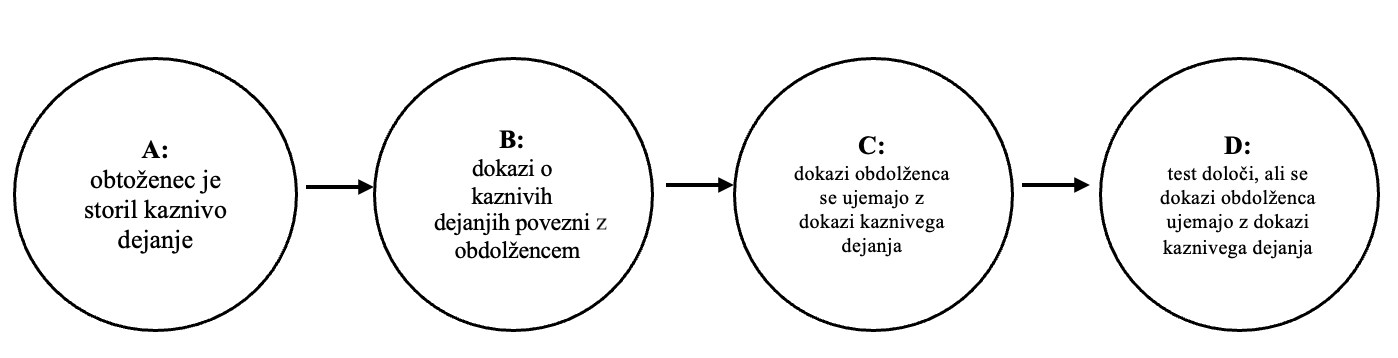
\includegraphics[scale=0.40]{slika_3.png}
        \caption{Vzorčna veriga dokazov}
    \end{figure}
\end{frame}

\begin{frame}
    \frametitle{Zmote v kazenskem pravu}
    \begin{block}{Zmota odvisnih dokazov}
        dva ali več dokazov, ki so odvisni, obravnavamo, kot da bi bili neodvisni. \\
        Poseben primer te zmote je \textit{logično odvisna dokazna zmota}.\\ \vspace{2mm}
    \end{block} \vspace{2mm}
    \begin{block}{Napaka konjunkcije}
        preiskovalec ne upošteva dejstva, da je dokaz sestavljen iz več kot enega negotovega dogodka, in mu posledično pripiše večjo verjetnost, kot bi jo moral.
    \end{block}
\end{frame}

%%%%%%%%%%%%%%%%%%%%%%%%%%%%%%%%%%%%%%%%%%%%%%%%%%%%%%%%%%%%%%%%%%%%%%%%%%%%%%%%%%%%%%%%%%%%%%%%%%%%%%%%%%%%%%%%%%%%%%%%%%%%%%%%%%%%%%%%%%%%
%%%%%%%%%%%%%%%%%%%%%%%%%%%%%%%%%%%%%%%%%%%%%%%%%%%%%%%%%%%%%%%%%%%%%%%%%%%%%%%%%%%%%%%%%%%%%%%%%%%%%%%%%%%%%%%%%%%%%%%%%%%%%%%%%%%%%%%%%%%%
\section{Načini za izogib zmotam}

\begin{frame}
    \frametitle{Izogib zmotam z uporabo razmerja verjetnosti}
    \begin{block}{Prednost uporabe razmerja verjetnosti}
        odpravlja ugovor Bayesovemu izreku, in sicer upoštevanje predhodne verjetnosti za hipotezo, kot je »kriv«.
    \end{block}\vspace{3mm}
    \centering
    $\Rightarrow$ težave pri razumevanju razmerja verjetnosti kot pri razumevanju Bayesove teorije
\end{frame}

%%%%%%%%%%%%%%%%%%%%%%%%%%%%%%%%%%%%%%%%%%%%%%%%%%%%%%%%%%%%%%%%%%%%%%%%%%%%%%%%%%%%%%%%%%%%%%%%%%%%%%%%%%%%%%%%%%%%%%%%%%%%%%%%%%%%%%%%%%%%
\begin{frame}
    \frametitle{Izogibanje zmotam z uporabo Bayesovih omrežij}
    \begin{block}{}
        Bayesova omrežja pomagajo določiti ustrezne verjetnostne formule, ne da bi prikazali njihovo polno algebrsko obliko, in omogočajo skoraj popolno avtomatizacijo potrebnih verjetnostnih izračunov.
    \end{block} \vspace{3mm}
    \begin{enumerate}
        \item med konkurenčnimi hipotezami izbramo najverjetnejšo;
        \item izbira mora biti podprta z znanstveno utemeljeno argumentacijo;
        \item primerna so za analizo dogodka;
        \item primern za napovedovanje verjetnosti, da je k dogodku prispeval katerikoli od več možnih
        znanih vzrokov;
    \end{enumerate}
    \begin{block}{}
        Prednosti Bayesovih mrež se najbolj izrazito pokažejo na zapletenih področjih z več spremenljivkami.
    \end{block}
\end{frame}

\begin{frame}
    \frametitle{Izogibanje zmotam z uporabo Bayesovih omrežij}
    \begin{itemize}
        \item bistveno izboljšajo vrednotenje verjetnostnih razmerij, ki se uporabljajo za ocenjevanje znanstvenih dokazov;
        \item omogočajo kompleksnejše verjetnostne analize;
        \item če se za izdelavo ne uporablja dosleden okvir, lahko Bayesovo omrežje kaže različne rezultate;
    \end{itemize} \vspace{3mm}
    \begin{block}{}
        Prikaz Bayesovega omrežja se mora ujemati z intuitivnim pripisovanjem vzročno-posledičnih povezav med končno hipotezo, podhipotezo in dokazi primera.
    \end{block}
\end{frame}

%%%%%%%%%%%%%%%%%%%%%%%%%%%%%%%%%%%%%%%%%%%%%%%%%%%%%%%%%%%%%%%%%%%%%%%%%%%%%%%%%%%%%%%%%%%%%%%%%%%%%%%%%%%%%%%%%%%%%%%%%%%%%%%%%%%%%%%%%%%%
%%%%%%%%%%%%%%%%%%%%%%%%%%%%%%%%%%%%%%%%%%%%%%%%%%%%%%%%%%%%%%%%%%%%%%%%%%%%%%%%%%%%%%%%%%%%%%%%%%%%%%%%%%%%%%%%%%%%%%%%%%%%%%%%%%%%%%%%%%%%

\end{document}